\documentclass[crop,class=article]{standalone}
%----------------------------Preamble-------------------------------%
\usepackage{tikz}                       % Drawing/graphing tools.
%--------------------------Main Document----------------------------%
\begin{document}
    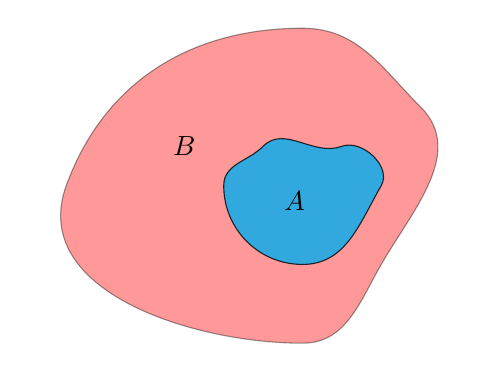
\begin{tikzpicture}
        \draw[fill=red, opacity=0.4] (0,-2) to [out=0,in=-120] (1,-1)
                                            to [out=60,in=-45] (1.5,1)
                                            to [out=135,in=0] (0,2)
                                            to [out=-180,in=70] (-3,0)
                                            to [out=-110,in=-180] cycle;
        \draw[fill=cyan, opacity=0.8]
            (0,-1) to [out=0,in=-120] (1,0)
                   to [out=60,in=20] (0.5,0.5)
                   to [out=-160,in=45] (-0.5,0.5)
                   to [out=-135,in=90] (-1,0)
                   to [out=-90,in=180] cycle;
        \node at (-0.1,-0.2) {$A$};
        \node at (-1.5,0.5) {$B$};
    \end{tikzpicture}
\end{document}